% Advanced Beamer Presentation - Complete Tutorial Example
% Based on Dr. Trefor Bazett's YouTube Tutorial
% Video URL: https://www.youtube.com/watch?v=rx7wwtmFlD8

% 1. Setup: Document class with widescreen aspect ratio [09:18]
\documentclass[aspectratio=169]{beamer}

% Optional: Handout mode for printing (uncomment for handouts) [19:51]
% \documentclass[aspectratio=169,handout]{beamer}
% \usepackage{pgfpages}
% \pgfpagesuselayout{4 on 1}[letterpaper,border shrink=5mm]

% Required packages
\usepackage{amsmath,amsfonts,amssymb,amsthm}
\usepackage{tikz}
\usetikzlibrary{shapes,arrows,positioning}

% 3. Visual Enhancements and Theming
% Theme and color theme [09:40]
\usetheme{Copenhagen}
\usecolortheme{beaver}

% Transparency option to show upcoming content as faint text [11:44]
\setbeamercovered{transparent}

% Remove navigation symbols for cleaner look
\setbeamertemplate{navigation symbols}{}

% Title information
\title{Advanced Beamer Presentation}
\subtitle{A Complete Tutorial Example}
\author{LaTeX Research Toolkit}
\institute{Based on Dr. Trefor Bazett's Tutorial}
\date{\today}

\begin{document}

% Title slide
\begin{frame}
  \titlepage
\end{frame}

% 4. Navigation: Table of Contents [18:33]
\begin{frame}{Table of Contents}
  \tableofcontents
\end{frame}

% 4. Navigation: Sections [16:43]
\section{Basic Frames and Structure}

% 1. Basic Structure: Individual slides using frame environment [03:13]
\begin{frame}{Welcome to Beamer}
  This is a basic frame with a title and content.
  
  \vspace{0.5cm}
  
  Frames are the building blocks of Beamer presentations. Each frame can contain:
  \begin{itemize}
    \item Text content
    \item Lists (itemize, enumerate)
    \item Mathematical formulas
    \item Graphics and tables
    \item And much more!
  \end{itemize}
\end{frame}

\section{Animation and Overlays}

% 2. Controlling Content Flow: Incremental Display [04:37]
\begin{frame}{Incremental Lists with Overlays}
  Using angle brackets to control when items appear:
  
  \begin{itemize}
    \item<1-> This appears on slide 1 and remains visible
    \item<2-> This appears starting on slide 2
    \item<3-> This appears starting on slide 3
    \item<4-> All items remain visible once they appear
  \end{itemize}
  
  \vspace{0.5cm}
  \onslide<5->{
    \textbf{Note:} The syntax \texttt{<n->} means "from slide n onward"
  }
\end{frame}

% 2. Conditional Visibility: only vs onslide [06:03]
\begin{frame}{Conditional Visibility: \texttt{\textbackslash only} vs \texttt{\textbackslash onslide}}
  \textbf{Key Difference:}
  \begin{itemize}
    \item \texttt{\textbackslash only}: Content doesn't take up space when hidden (preferred)
    \item \texttt{\textbackslash onslide}: Content takes up space even when hidden
  \end{itemize}
  
  \vspace{0.5cm}
  
  \only<2>{
    \textcolor{blue}{\textbf{This text appears ONLY on slide 2 (using \textbackslash only)}}
  }
  \only<3>{
    \textcolor{red}{\textbf{This text appears ONLY on slide 3 (using \textbackslash only)}}
  }
  
  \vspace{0.5cm}
  
  \onslide<4->{
    This text is visible from slide 4 onward (using \texttt{\textbackslash onslide})
  }
\end{frame}

% 2. Aesthetics: alert and textbf for emphasis [07:46]
\begin{frame}{Highlighting and Emphasis}
  You can draw attention to specific points:
  
  \begin{itemize}
    \item<1-> Normal text on slide 1
    \item<2-> \alert<2>{This text is alerted on slide 2 only}
    \item<3-> \textbf<3>{This text is bold on slide 3 only}
    \item<4-> \alert{This text is always alerted}
  \end{itemize}
  
  \vspace{0.5cm}
  
  \only<5>{
    \begin{center}
      \Large \alert{\textbf{You can combine \textbackslash alert and \textbackslash textbf!}}
    \end{center}
  }
\end{frame}

\section{Special Environments}

% 4. Advanced Elements: Special Environments [12:25]
\begin{frame}{Block Environments}
  Beamer provides several special environments with automatic styling:
  
  \begin{block}{Standard Block}
    This is a standard block environment. It's useful for emphasizing content.
  \end{block}
  
  \begin{example}
    This is an example environment. Perfect for demonstrating concepts.
  \end{example}
  
  \begin{alertblock}{Alert Block}
    This is an alert block. Use it for warnings or important notes.
  \end{alertblock}
\end{frame}

\begin{frame}{Theorems and Proofs}
  Mathematical content with proper formatting:
  
  \begin{theorem}[Pythagorean Theorem]
    In a right triangle, $a^2 + b^2 = c^2$ where $c$ is the length of the hypotenuse.
  \end{theorem}
  
  \begin{proof}
    Consider a right triangle with sides $a$, $b$, and hypotenuse $c$.
    
    By constructing squares on each side, we can show through geometric decomposition that the area of the square on the hypotenuse equals the sum of the areas of the squares on the other two sides.
    
    Therefore, $c^2 = a^2 + b^2$.
  \end{proof}
  
  \textbf{Note:} The QED symbol ($\square$) appears automatically at the end of proofs.
\end{frame}

\section{Columns and Layout}

% 4. Advanced Elements: Columns [14:26]
\begin{frame}{Two-Column Layout}
  \begin{columns}
    \begin{column}{0.48\textwidth}
      \textbf{Left Column:}
      \begin{itemize}
        \item Columns are useful for organizing content
        \item You can put text, lists, or graphics
        \item Each column has independent formatting
      \end{itemize}
    \end{column}
    
    \begin{column}{0.48\textwidth}
      \textbf{Right Column:}
      \begin{enumerate}
        \item First numbered item
        \item Second numbered item
        \item Third numbered item
      \end{enumerate}
    \end{column}
  \end{columns}
\end{frame}

\begin{frame}{Columns with TikZ Graphics}
  \begin{columns}
    \begin{column}{0.5\textwidth}
      \textbf{Text and Description:}
      
      TikZ allows you to create beautiful diagrams directly in LaTeX.
      
      \vspace{0.3cm}
      
      The diagram on the right shows a simple flowchart with three connected nodes.
      
      \vspace{0.3cm}
      
      This is perfect for presenting algorithms or processes.
    \end{column}
    
    \begin{column}{0.5\textwidth}
      \begin{center}
        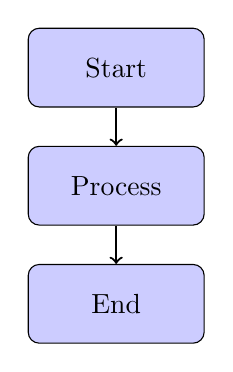
\begin{tikzpicture}[node distance=1.5cm,
          box/.style={rectangle, draw, fill=blue!20, text width=2cm, text centered, rounded corners, minimum height=1cm}]
          
          \node[box] (start) {Start};
          \node[box, below of=start] (process) {Process};
          \node[box, below of=process] (end) {End};
          
          \draw[->, thick] (start) -- (process);
          \draw[->, thick] (process) -- (end);
        \end{tikzpicture}
      \end{center}
    \end{column}
  \end{columns}
\end{frame}

\begin{frame}{Columns with Mathematics}
  \begin{columns}
    \begin{column}{0.5\textwidth}
      \textbf{Matrix Operations:}
      
      Consider two matrices $A$ and $B$:
      
      \[
      A = \begin{pmatrix}
        1 & 2 \\
        3 & 4
      \end{pmatrix}
      \]
    \end{column}
    
    \begin{column}{0.5\textwidth}
      \[
      B = \begin{pmatrix}
        5 & 6 \\
        7 & 8
      \end{pmatrix}
      \]
      
      \vspace{0.3cm}
      
      Their product is:
      \[
      AB = \begin{pmatrix}
        19 & 22 \\
        43 & 50
      \end{pmatrix}
      \]
    \end{column}
  \end{columns}
\end{frame}

\section{Combined Features}

\begin{frame}{Combining Overlays with Columns}
  \begin{columns}
    \begin{column}{0.5\textwidth}
      \textbf{Progressive Revelation:}
      \begin{itemize}
        \item<1-> First point appears
        \item<2-> Second point appears
        \item<3-> Third point appears
      \end{itemize}
    \end{column}
    
    \begin{column}{0.5\textwidth}
      \only<1>{
        \begin{block}{Step 1}
          Initial information shown with first point.
        \end{block}
      }
      \only<2>{
        \begin{block}{Step 2}
          Additional details with second point.
        \end{block}
      }
      \only<3>{
        \begin{alertblock}{Step 3}
          Final conclusion with third point!
        \end{alertblock}
      }
    \end{column}
  \end{columns}
\end{frame}

\begin{frame}{Combining Blocks and Overlays}
  \only<1>{
    \begin{block}{Question}
      What is the derivative of $f(x) = x^2$?
    \end{block}
  }
  
  \only<2->{
    \begin{block}{Question}
      What is the derivative of $f(x) = x^2$?
    \end{block}
    
    \begin{example}<2->
      Using the power rule: $f'(x) = 2x$
    \end{example}
  }
  
  \only<3>{
    \begin{alertblock}{Verification}
      We can verify: $\lim_{h \to 0} \frac{(x+h)^2 - x^2}{h} = \lim_{h \to 0} \frac{2xh + h^2}{h} = 2x$ \checkmark
    \end{alertblock}
  }
\end{frame}

\section{Summary and Conclusion}

\begin{frame}{Summary of Beamer Features}
  This presentation demonstrated:
  
  \begin{enumerate}
    \item<1-> \textbf{Setup:} Document class with widescreen format (16:9)
    \item<2-> \textbf{Overlays:} Incremental display using angle brackets
    \item<3-> \textbf{Visibility:} \texttt{\textbackslash only} vs \texttt{\textbackslash onslide}
    \item<4-> \textbf{Emphasis:} \texttt{\textbackslash alert} and \texttt{\textbackslash textbf}
    \item<5-> \textbf{Themes:} Copenhagen theme with beaver colors
    \item<6-> \textbf{Transparency:} Faint preview of upcoming content
    \item<7-> \textbf{Environments:} Blocks, examples, theorems, and proofs
    \item<8-> \textbf{Columns:} Multi-column layouts with text and graphics
    \item<9-> \textbf{Navigation:} Sections and table of contents
    \item<10-> \textbf{Handouts:} Optional multi-slide-per-page printing
  \end{enumerate}
\end{frame}

\begin{frame}{Tips for Creating Great Presentations}
  \begin{block}{Design Principles}
    \begin{itemize}
      \item Keep slides simple and uncluttered
      \item Use overlays to guide audience attention
      \item Choose themes that match your content
      \item Leverage special environments for clarity
    \end{itemize}
  \end{block}
  
  \begin{alertblock}{Remember}
    The goal is effective communication, not just fancy effects!
  \end{alertblock}
\end{frame}

\begin{frame}{Additional Resources}
  \textbf{Learn More:}
  \begin{itemize}
    \item Overleaf Beamer Documentation: \url{https://www.overleaf.com/learn/latex/Beamer}
    \item Beamer Theme Gallery: \url{https://deic.uab.cat/~iblanes/beamer_gallery/}
    \item Dr. Trefor Bazett's Tutorial: \url{https://www.youtube.com/watch?v=rx7wwtmFlD8}
  \end{itemize}
  
  \vspace{0.5cm}
  
  \textbf{To create handouts:}
  \begin{itemize}
    \item Uncomment the handout option in the document class
    \item Uncomment the pgfpages configuration
    \item Recompile to get 4 slides per page
  \end{itemize}
\end{frame}

\begin{frame}
  \begin{center}
    {\Huge Thank You!}
    
    \vspace{1cm}
    
    {\Large Questions and Discussion}
    
    \vspace{1cm}
    
    \small
    This advanced example covers all major Beamer features\\
    from Dr. Trefor Bazett's comprehensive tutorial.
  \end{center}
\end{frame}

\end{document}
